\documentclass[11pt]{article}
\usepackage{amsmath,amsfonts,amssymb,algorithm,algpseudocode}
\usepackage{graphicx,tikz,setspace}
\usepackage[hidelinks]{hyperref}
\usepackage[mathscr]{euscript}
\usepackage[top=1in, left=1.5in, right=1.5in, bottom=1in]{geometry}

\newcommand{\pd}[2]{\frac{\partial #1}{\partial #2}}
\setstretch{1.5}

\title{Practicum in Artificial Intelligence:\\ Optical Character Recognition via Neural Networks}
\date{December 12, 2012}
\author{Bryan Cuccioli (\texttt{blc72@cornell.edu}), Mathematics \& Computer Science, 2014\\
\and
Renato Amez (\texttt{ra374@cornell.edu}), Electrical \& Computer Engineering, 2014}

\usetikzlibrary{calc,positioning,arrows,chains,decorations.pathreplacing,matrix}

\tikzset{
>=stealth',
  punktchain/.style={
    rectangle, 
    rounded corners, 
    fill=black!5,
    draw=black, very thick,
    text width=9em, 
    minimum height=3em, 
    text centered, 
    on chain},
  line/.style={draw, thick, <-},
  element/.style={tape, text centered, on chain},
  every join/.style={->, thick,shorten >=1pt},
  decoration={brace},
  tuborg/.style={decorate},
  tubnode/.style={midway, right=2pt},
}

\begin{document}

\maketitle
\tableofcontents
\pagebreak

\section{Abstract}

\emph{
We propose to design and train a feed-forward, multilayer neural network with back-propagation to perform optical character recognition. We give a formal definition of the problem of optical character recognition, and then exhibit the design and topology of such a neural network. We present experimental results relating several construction parameters, such as number of hidden layers, response threshold, and learning rate, independently to the output of our neural network.
}

\section{Introduction}
Optical character recognition (OCR) is an important problem in computer vision, with applications ranging from efficiently scanning books to recognizing cheques in an ATM. We aim to give a simple solution to the problem of OCR via training a neural network. In particular, we approximately model the human brain as a weighted directed graph and use training samples to tune the weights, enabling the network to compute the character corresponding to the representation in an image. This gives a relatively simple version of a general purpose \emph{linear classifier}, more sophisticated versions of which are used in industry to perform OCR.

We exhibit the design and structure of such a network, and experimentally determine parameters of its construction that give optimal results.

\subsection{Formal Description}

We will now give a more precise definition of the problem of optical character recognition. Each image in our input set is of size $N\times N$, consisting of pixel values in $\{0,\dots,M\}$, and represents a digit between 0 and 9. That is, each image is a vector in the $N\times N$-dimensional vector space $\mathscr{V}$ taken over the Galois field $\mathbf{F}=\mathrm{GF}(M+1)$. We aim to construct a function
\begin{equation}\varphi:\mathscr{V}\xrightarrow{\ \ \ } \{0,1,\dots,9\}\end{equation}
that assigns to each image $v\in\mathscr{V}$ an output $n\in \{0,1,\dots,9\}$, such that the output corresponds to the digit represented in the image.

\section{Method}

Our method for solving this problem is to create a multi-layer feed-forward neural network trained with back-propagation. A \emph{neural network} is a directed weighted graph $G=(V,E)$ such that the set of \emph{neurons} $V$ is partitioned into a set of \emph{layers} $\{L_1,\dots,L_n\}$, with $n\geq 2$. The layer $L_1$ is called the \emph{input layer}, and $L_n$ the \emph{output layer}; the remaining layers are \emph{hidden layers}, and all have the same cardinality. For each $i=1,\dots,n-1$, we form the edge set between layers
\[E_i=\{(u,v) : u\in L_i\mathrm{\ and\ } v\in L_{i+1}\}\]
so that our neural network has edges
\begin{equation}E=\bigcup_{i=1}^{n-1} E_i.\end{equation}
We also add to each layer a \emph{bias node}, and create an edge from this node to every neuron in the layer.

For example, Figure \ref{nn} shows a simple neural network with two hidden layers, each containing five neurons, an input layer containing four neurons, and an output layer containing three neurons, with no bias node.

\def\layersep{2.5cm}

\vspace{1cm}
\begin{figure}[h]
\centering
\begin{tikzpicture}[shorten >=1pt,->,draw=black!50, node distance=\layersep]
    \tikzstyle{every pin edge}=[<-,shorten <=1pt]
    \tikzstyle{neuron}=[circle,fill=black,minimum size=6pt,inner sep=0pt]
    \tikzstyle{input neuron}=[neuron];
    \tikzstyle{output neuron}=[neuron];
    \tikzstyle{hidden neuron}=[neuron];
    \tikzstyle{annot} = [text width=4em, text centered]

    % Draw the input layer nodes
    \foreach \name / \y in {1,...,4}
        \node[input neuron, pin=left:Input \#\y] (I-\name) at (0,-\y) {};

    % Draw the hidden layer nodes
    \foreach \name / \y in {1,...,5}
        \path[yshift=.5cm]
            node[hidden neuron] (H1-\name) at (\layersep,-\y cm) {};
    \foreach \name / \y in {1,...,5}
        \path[yshift=.5cm]
            node[hidden neuron] (H2-\name) at (5cm,-\y cm) {};

    % Draw the output layer nodes
    \node[output neuron,pin={[pin edge={->}]right:Output}, right of=H2-2] (O1) {};
    \node[output neuron,pin={[pin edge={->}]right:Output}, right of=H2-3] (O2) {};
    \node[output neuron,pin={[pin edge={->}]right:Output}, right of=H2-4] (O3) {};

    % Connect every node in the input layer with every node in the
    % hidden layer.
    \foreach \source in {1,...,4}
        \foreach \dest in {1,...,5}
            \path (I-\source) edge (H1-\dest);

    % Connect every node between the hidden layers
    \foreach \source in {1,...,5}
        \foreach \dest in {1,...,5}
            \path (H1-\source) edge (H2-\dest);

    % Connect every node in the hidden layer with the output layer
    \foreach \dest in {1,...,3}
        \foreach \source in {1,...,5}
            \path (H2-\source) edge (O\dest);

    % Annotate the layers
    \node[annot,above of=H1-1, node distance=1cm] (hl) {Hidden layer};
    \node[annot,above of=H2-1, node distance=1cm] (hl2) {Hidden layer};
    \node[annot,left of=hl] {Input layer};
    \node[annot,right of=hl2] {Output layer};
\end{tikzpicture}
\caption{Topology of a simple neural network} \label{nn}
\end{figure}
\vspace{1cm}

We begin by initializing each edge weight to a random value in the interval $[-10,10]$. We then \emph{feed forward} each input in the neural network to compute the output. This is done by computing for each neuron the weighted sum of its inputs, and then passing to the \emph{sigmoid function} $\sigma:\mathbb{R}\xrightarrow{\ \ \ \ } \mathbb{R}_{\geq 0}$ given by
\begin{equation}\sigma(x) = \frac{1}{1+e^{-x/a}},\end{equation}
where $a$ is the \emph{activation threshold}. The function $\sigma$ approximates an activation threshold to the perceptron, and has the advantage of being differentiable, which is necessary for the back-propagation step.

For each $i=2,\dots,n$ in sequence, we compute for each neuron $j$
\begin{equation}b_j = \sum_{k=1}^m w_{k,j} a_k, \mathrm{\ \ \ } a_j=\sigma(b_j),\end{equation}
where $m$ is the number of neurons in each hidden layer, $w_{k,j}$ is the weight of the edge $(k,j)$, and the $a_k$ are initialized in the input layer to the values of the inputs. This is exhibited fully in Algorithm 1.

\begin{algorithm}
\caption{Feed forward}
\begin{algorithmic}[1]
\Function{FeedForward}{input $(x_1,x_2,\dots,x_r)$}
\For{node $i$ in the input layer}
  \State $a_i \gets x_i$
\EndFor
\For{$\ell=2,...,n$}
  \For{node $j$ in layer $\ell$}
    \State $b_j\gets \sum_i w_{i,j} a_i$
    \State $a_j \gets \sigma(b_j)$
  \EndFor
\EndFor
\State \Return set of neurons in $L_n$
\EndFunction
\end{algorithmic}
\end{algorithm}

To facilitate learning in the neural network, it is necessary to update the edge weights after computing the output based on whether the output was correct. The process by which this is accomplished is called \emph{back-propagation}. At a high level, the idea behind the back-propagation algorithm is that we can update the weights in the edges of $E_{n-1}$ in order to minimize the \emph{loss}, a heuristic designed to measure the distance between the output and the desired output. This gives the desired activation values for the neurons of layer $L_{n-1}$, so we update the weights of edges in $E_{n-2}$ similarly, and recurse until the input layer is reached. 

We will derive and analyze a method for computing the updated weights. Suppose that $\mathbf{a}=(a_1,\dots,a_s)$ is the input vector, and $\mathbf{y}=(y_1,\dots,y_r)$ is the desired output. Let $f$ be the function that implements the neural network, i.e. the function that takes in the input vector and weight vector $\mathbf{w}$ consisting of all of the weights in the network, and returns the output layer $f(\mathbf{a},\mathbf{w})$. Define the ``loss function'' $\mathscr{L}$ as
\begin{align}\mathscr{L}(\mathbf{a})&=\sum_{i=1}^r (y_i - f(a_i,\mathbf{w}))^2\notag\\
&=\sum_{i=1}^r \mathscr{L}_i(\mathbf{a}).\end{align}

We implement back-propagation as a form of hill-climbing search, following the gradient of the loss function in order to arrive at a local minimum. We begin by defining for each node $j$ in the output layer
\begin{equation}\Delta_j = \sigma'(b_j) \cdot (y_j-a_j).\end{equation}
Then observe that at the output layer, we can compute the gradient of $\mathscr{L}_k$ as
\begin{align}\pd{\mathscr{L}_k}{w_{j,k}} &= -2(y_k-a_k)\pd{a_k}{w_{j,k}}\notag\\
&=-2(y_k-a_k)\pd{\sigma(b_k)}{w_{j,k}}\notag\\
&=-2(y_k-a_k)\sigma'(b_k)\pd{b_k}{w_{j,k}}\notag\\
&=-2(y_k-a_k)\sigma'(b_k)\pd{}{w_{j,k}} \left(\sum_{j} w_{j,k} a_j\right)\notag\\
&=-2(y_k-a_k)\sigma'(b_k)a_j\notag\\&=-a_j \Delta_k.\end{align}
The gradients with respect to the weights in layers upstream from the output layer can now be computed. For each $i=n-1,\dots,1$, we define for each neuron $j\in L_i$,
\begin{equation}\Delta_j = \sigma'(a_j) \sum_{k\in L_{i+1}} w_{j,k} \Delta_k,\end{equation}
so that
\begin{align}\pd{\mathscr{L}_k}{w_{i,j}} &= -2(y_k-a_k)\pd{a_k}{w_{i,j}}\notag\\
&=-2(y_k-a_k)\pd{\sigma(b_k)}{w_{i,j}}\notag\\
&=-2(y_k-a_k)\sigma'(b_k)\pd{b_k}{w_{i,j}}\notag\\
&=-2\Delta_k \pd{}{w_{i,j}} \left(\sum_j w_{j,k} a_j\right)\notag\\
&=-2\Delta_k w_{j,k} \pd{a_j}{w_{i,j}}\notag\\
&=-2\Delta_k w_{j,k} \sigma'(b_j) \pd{b_j}{w_{i,j}}\notag\\
&=-2\Delta_k w_{j,k} \sigma'(b_j) \pd{}{w_{i,j}}\left(\sum_i w_{i,j} a_i\right)\notag\\
&=-2\Delta_k w_{j,k} \sigma'(b_j) a_i\notag\\
&=-a_i \Delta_j.\end{align}
Hence it remains to update each edge weight by adding the gradient of the loss function at that weight, multiplied by some pre-defined \emph{learning rate} $\lambda$. The full back-propagation algorithm is shown in Algorithm 2.

\begin{algorithm}
\caption{Back-propagate}
\begin{algorithmic}[1]
\Function{BackPropagate}{output $\mathbf{a}$, correct output $\mathbf{y}$}
\For{node $j$ in the output layer}
  \State $\Delta_j \gets \sigma'(b_j)\cdot (y_j-a_j)$
\EndFor
\For{$\ell=n-1,\dots,1$}
  \For{node $i$ in layer $\ell$}
    \State $\Delta_i\gets \sigma'(b_i) \sum_{j\in L_{\ell+1}} w_{i,j}\Delta_j$
  \EndFor
\EndFor
\For{weight $w_{i,j}$ in network}
  \State $w_{i,j}\gets w_{i,j} + \lambda\times a_i\times \Delta_j$
\EndFor
\EndFunction
\end{algorithmic}
\end{algorithm}

At the top level, we use $t$ training examples per digit, computing the output through the neural network in each and then back-propagating in turn to update the weights. Each image is first resized from $28\times 28$ to $6\times 6$, and is then converted from grayscale to black and white using Otsu thresholding. This serves to reduce the dimensionality of the input, so that the input set can be fit more accurately to the weights. We construct a neural network with $6\times 6$ neurons in the input layer, each corresponding to a pixel in the image, and 10 neurons in the output layer, each corresponding to a possible output $0,1,\dots,9$, with activation values $a_i$ representing the network's confidence that $i$ is the correct output.

We then execute the training algorithm shown in Algorithm 3.

\begin{algorithm}
\caption{Train}
\begin{algorithmic}[1]
\Function{Train}{training set $S$}
\For{weight $w_{i,j}$ in $\mathbf{w}$}
  \State $w_{i,j} \gets \mathrm{\ small\ random\ value}$
\EndFor
\For{image $s\in S$}
  \State $s\gets \mathrm{resize}(s)$
  \State $f(\mathbf{s},\mathbf{w})\gets \mathrm{FeedForward}(\mathbf{s})$
  \State BackPropagate($f(\mathbf{s},\mathbf{w})$, desired output)
\EndFor
\EndFunction
\end{algorithmic}
\end{algorithm}

The \emph{success} of the neural network is measured by running the above algorithm on some distinct set of $T$ images without the BackPropagate stage and counting for how many images the correct value was output.

\section{System Architecture}

The implementation of the system is divided among four main classes. Although an approach not based on object-oriented programming using only a three-dimensional array to store weights and activation values is possible, the structure of a neural network and modularization of the project lend themselves well to a class-based approach.

\begin{enumerate}
\item \texttt{ImageData}: This class is responsible for reading in images from the data set, resizing them, and thresholding them from grayscale to black and white. Image processing is done via the OpenCV \footnote{\url{http://opencv.org}} library.

\item \texttt{Neuron}: This class represents a single neuron in the network. Each neuron stores its activation value and the weights of its incoming edges. It handles the logic for randomly assigning values to these weights upon initialization as well as for computing the linear combination of its inputs.

\item \texttt{Layer}: This class represents a layer of the neural network. It stores an array of neurons belonging to this layer, and handles the logic for initializing each neuron.

\item \texttt{NeuralNet}: This class represents the neural network at the top level. It handles the logic for initializing each layer and implements the FeedForward and BackPropagate algorithms.
\end{enumerate}

\vspace{.5cm}
\begin{figure}[h]
\centering
\begin{tabular}{ccc}
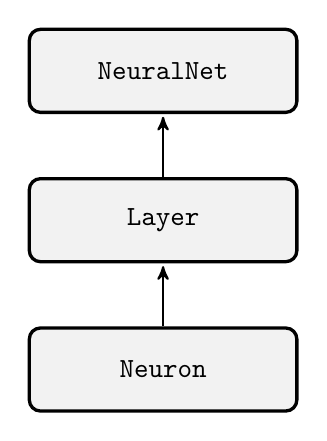
\begin{tikzpicture}
  [node distance=.8cm, start chain=going above,]
  \node[punktchain, join] (neuron) {\texttt{Neuron}};
  \node[punktchain, join] (layer) {\texttt{Layer}};
  \node[punktchain, join] (neuralnet) {\texttt{NeuralNet}};
\end{tikzpicture}
& \hspace{.75cm} &
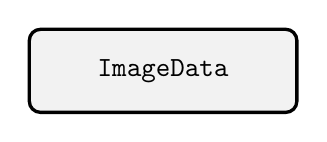
\begin{tikzpicture}
  [node distance=.8cm, start chain=going above,]
  \node[punktchain] (imagedata) {\texttt{ImageData}};
\end{tikzpicture}
\end{tabular}
\caption{Class structure} \label{classes}
\end{figure}
\vspace{.5cm}

Training and testing is done using Google's MNIST database \footnote{\url{http://yann.lecun.com/exdb/mnist/}}. As part of pre-processing, a simple C\# script\footnote{\url{https://gist.github.com/4056614}} was used to convert the glob of pixel values to 10,000 JPEG images suitable for processing. 

\section{Experimental Evaluation}

\subsection{Methodology}

The interface to the program supports specifying several variables that we test in relation to the success of the network, including

\begin{itemize}
\item $t$: the number of training samples per digit;
\item $\ell$: the number of hidden layers in the network;
\item $h$: the number of neurons per hidden layer;
\item $b$: the weight of the bias;
\item $\lambda$: the learning rate of the network, as defined above;
\item $r$: the response threshold for the sigmoid function.
\end{itemize}
We vary each of these parameters independently over several discrete values, holding fixed the size of the test sample set $T=100$. Training and test data samples are taken from the MNIST database, a collection of 10,000 handwritten digits. Recognizing digits simplifies the problem of learning optical character recognition without loss of generality; it can easiy be extended to learning to recognize all handwritten characters.

\subsection{Results}

The hypothesis established before beginning the experimental trials was that increasing every one of the above parameters separately would increase the success rate of the neural network roughly linearly. Experimental trials show that each of the parameters affects the output in this way between some lower and upper bound.

We found that the learning rate $\lambda$ is one such parameters which increases the success up to some upper bound. We fix $\ell=1$, $h=45$, $t=800$, $r=55$, and $b=60$. With $\lambda=1$, we get $\mu=10.3\% \pm 1.1\%$. With $\lambda=10$, we get $\mu=27.0\% \pm 1.3\%$. With $\lambda=40$, we get $\mu=34.4\% \pm 1.4\%$. However, with $\lambda=50$, we get $\mu=27.2\% \pm 1.2\%$, and the results similarly decrease from there, indicating that the optimal value for $\lambda$ is approximately 40.

We found that having one hidden layer is optimal for our neural network. With $\lambda=40$ and the other parameters fixed as above, we find that with $\ell=0$, we get $\mu=12.3\% \pm 1.3\%$. With $\ell=1$, we get $\mu=34.4\% \pm 1.4\%$, as above. With $\ell=2$, we get $\mu=23.8\% \pm 1.6\%$, and with $\ell=3$, we get $\mu=12.7\% \pm 0.8\%$. This makes intuitive sense: having too few nodes available should make it hard for the network to generalize to the entire dataset, while having too many subjects the network to \emph{overfitting}.

By the same reasoning, we intuit that there will be some middle value for $h$ that is optimal. Experimental results confirm this: with $h=25$ we get $\mu=15.7\% \pm 0.7\%$; with $h=45$ we get $\mu=30.4\% \pm 1.2\%$; with $h=55$, we get $\mu=35.1\% \pm 1.4\%$, and the outputs stay approximately constant up through at least $h=100$ (fixing the optimal values above for the other parameters).

We found that the response threshold $r$ greatly influences the success of the neural network. Fix the other parameters as above, with $h=45$. With $r=25$, we get $\mu=15.2\% \pm 2.2\%$; with $r=35$, we get $\mu=23.8\%\pm 2.0\%$; with $r=55$ we get $\mu=31.8\% \pm 1.6\%$; with $r=65$ however we get $\mu=20.0\% \pm 1.9\%$. Intuitively, it makes sense that having a value for $r$ that is slightly too large or too low can drastically affect the outcome, as it skews the already steep slope of the sigmoid curve.

The bias element also has a weak effect on the outcome. Having a bias $b=0$ gives an output $\mu=27.6\% \pm 1.6\%$; having a bias $b=20$ gives an output $\mu=28\%\pm 1.4\%$; we see that optimally the bias $b=60$ gives an output of $\mu=32.1\% \pm 2.0\%$; however, having a bias $b=70$ causes the output to drop to $\mu=21.3\% \pm 1.7\%$.

Finally, we observe that the number of training examples $t$ used has a strong effect on the success of the network, with diminishing returns. Fixing the other parameters with the above-determined values, with $t=200$ gives output $\mu=17.1\% \pm 1.8\%$; using $t=400$ gives output $\mu=29.2\%\pm 1.9\%$; with $t=600$ we have $\mu=31.2\%\pm 2.3\%$; with $t=900$ we have output $\mu=29.8\% \pm 2.2\%$, approximately the same result as with $t=600$. It is expected that the success of the neural network should level off as $t\to\infty$, since many of the training examples are very similar and eventually the weights are changing by very small amounts.

\section{Future Work}

The major shortcoming with using a neural network is that it does not achieve a high rate of recognition. While recognition rates in the neighborhood of 35\% indicate that the model is at least somewhat successful, it is unable to adapt the weights to the resolution required for 90\% or greater recognition. It appears that the neural network model is not general or adaptable enough to perform OCR effectively.

There are a number of methods from computer vision that can be used to increase the efficacy of OCR. For example, many commercial OCR solutions use feature detection mechanisms such as computing the Laplacian of a Gaussian convolved with the image and then compare local features using e.g. scale-invariant feature transform (SIFT) to measure similarity between images$^3$. These methods could be incorporated into future versions of the project.

The neural network can also be adapted to a more robust detection mechanism. In particular, one could train a network to recognize for each $i\in \{0,\dots,9\}$ whether an input simply represents $i$ or not, and then apply all 10 neural networks to determine the digit in the image.

\section{Conclusion}

By constructing a multilayer feed-forward neural network and training it using back-propagation, we are able to implement a simple classifier that recognizes handwritten digits with a non-trivial success rate of approximately 35\%. Via experimentation, we determined that our neural network optimally has one hidden layer containing $h=45$ neurons, uses approximately $t=600$ training examples per digit, has a response threshold of $r=55$, a bias of $b=60$, and a learning rate of $\lambda=40$. These results make intuitive sense, as they achieve an optimal balance between under- and over-fitting the data.

While the neural network alone was able to achieve a success rate indicating that it is learning, it was not able to achieve a practically-applicable success rate alone. We posit that a neural network in combination with feature detection and extraction algorithms will perform significantly better.

\section{References}

\begin{enumerate}
\item \emph{``OpenCV''}. Visited December 12, 2012. $<$\url{http://opencv.org}$>$.

\item Cortes, LeCun. \emph{``The MNIST Database of Handwritten Digits''}.\\
Visited December 12, 2012. $<$\url{http://yann.lecun.com/exdb/mnist/}$>$.

\item Szeliski, Richard. \emph{Computer Vision: Algorithms and Applications.}\\ New York: SpringerLink, 2011.

\end{enumerate}

\section{Appendix: Code Tree}

\begin{itemize}
\item \texttt{main.cpp}: The main driver program, implements the top-level algorithm.

\item \texttt{Neuron.h}: Defines the \texttt{Neuron} class, contains logic for initializing a neuron and computing its activation.

\item \texttt{Layer.h}: Defines the \texttt{Layer} class, contains logic for initializing a layer of neurons.

\item \texttt{NeuralNet.h}: Defines an interface for the variables and methods of the \texttt{NeuralNet} class.

\item \texttt{NeuralNet.cpp}: Implements forward-feeding and back-propagation for the \texttt{NeuralNet} class.

\item \texttt{ImageData.h}: Defines an interface for the \texttt{ImageData} class, which handles processing of JPEG images into suitable pixel arrays.

\item \texttt{ImageData.cpp}: Implements the methods of the \texttt{ImageData} class.

\item \texttt{Makefile}: Build system used for compiling the project.
\end{itemize}

\end{document}
